\documentclass[border=10pt]{standalone}
\usepackage{pgfplots}
\pgfplotsset{compat=1.18}
\begin{document}
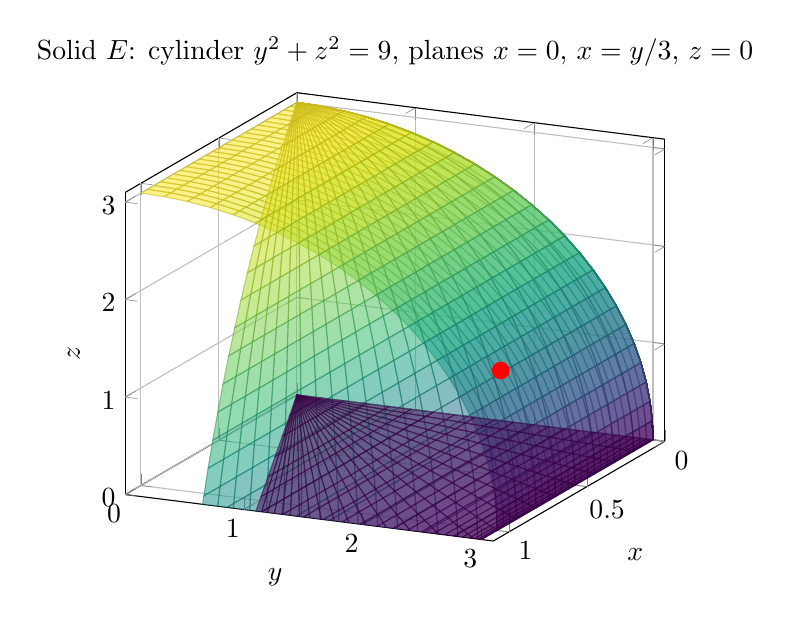
\begin{tikzpicture}
\begin{axis}[
    view={115}{20},
    xlabel={$x$}, ylabel={$y$}, zlabel={$z$},
    xmin=0, xmax=1.1, ymin=0, ymax=3.1, zmin=0, zmax=3.1,
    domain=0:1, y domain=0:90,
    colormap/viridis,
    grid,
    title={Solid $E$: cylinder $y^2+z^2=9$, planes $x=0$, $x=y/3$, $z=0$},
]
% Curved side: quarter cylinder y^2+z^2=9, param (x, y, z) = (s, 3 sin t, 3 cos t), s in [0, sin t]
\addplot3[surf, shader=faceted, opacity=0.55, z buffer=sort]
({x}, {3*sin(y)}, {3*cos(y)});
% Top slanted face x = y/3 over the quarter disk
\addplot3[surf, shader=faceted, opacity=0.55, z buffer=sort]
({x*3*sin(y)}, {3*sin(y)}, {3*cos(y)});
% Bottom face z = 0
\addplot3[surf, shader=faceted, opacity=0.5, z buffer=sort]
({x*3*sin(y)}, {3*sin(y)}, {0});
% Back face x = 0
\addplot3[surf, shader=faceted, opacity=0.5, z buffer=sort]
(0, {3*sin(y)}, {3*cos(y)});
% Center of mass marker
\addplot3[only marks, mark=*, mark size=3, color=red]
coordinates {(0.3747, 2.2089, 0.9375)};
\end{axis}
\end{tikzpicture}
\end{document}
